\documentclass[11pt,a4paper]{article}

% Standard packages
\usepackage[utf8]{inputenc}
\usepackage[T1]{fontenc}
\usepackage{amsmath,amssymb,amsthm}
\usepackage{mathtools}
\usepackage{graphicx}
\usepackage{float}
\usepackage{booktabs}
\usepackage{array}
\usepackage{enumitem}
\usepackage{hyperref}
\usepackage{cleveref}
\usepackage{geometry}
\usepackage{fancyhdr}
\usepackage{tikz}
\usetikzlibrary{arrows.meta,calc,decorations.markings,patterns,shapes.geometric,positioning}

\geometry{margin=2.5cm}

% Header/footer
\pagestyle{fancy}
\fancyhf{}
\fancyhead[L]{Bridge Paper 4}
\fancyhead[R]{L. Smart}
\fancyfoot[C]{\thepage}
\renewcommand{\headrulewidth}{0.4pt}

% Theorem environments
\newtheorem{theorem}{Theorem}[section]
\newtheorem{proposition}[theorem]{Proposition}
\newtheorem{lemma}[theorem]{Lemma}
\newtheorem{corollary}[theorem]{Corollary}
\newtheorem{definition}[theorem]{Definition}
\newtheorem{remark}[theorem]{Remark}
\newtheorem{assumption}[theorem]{Assumption}

% Custom commands (explicit definitions, no physics package)
\newcommand{\Egeom}{E_{\text{geom}}}
\newcommand{\Meff}{M_{\text{eff}}}
\newcommand{\Mgrav}{M_{\text{grav}}}
\newcommand{\Leff}{\mathcal{L}_{\text{eff}}}
\newcommand{\Geff}{G_{\text{eff}}}
\newcommand{\rhogeom}{\rho_{\text{geom}}}
\newcommand{\PhiG}{\Phi_G}
\newcommand{\dd}{\mathrm{d}}
\newcommand{\affmark}{\ensuremath{{}^*}}
\newcommand{\order}[1]{\mathcal{O}\left(#1\right)}

\begin{document}

\begin{titlepage}
\centering
\vspace*{2cm}

{\LARGE\bfseries On the Effective Dynamics of Stabilised Geometry\\[0.3cm] in Emergent Gravity Frameworks}

\vspace{0.5cm}
{\Large BP4}

\vspace{1.5cm}

{\large Lee Smart}\\[0.3cm]
{\itshape Vibrational Field Dynamics Institute}\\[0.2cm]
Email: contact@vibrationalfielddynamics.org\\
X (Twitter): @vfd\_org

\vspace{1cm}

December 4, 2025

\vspace{1.5cm}

\begin{abstract}
\noindent
Bridge Paper 3 established that gravity emerges as an effective curvature response to geometric non-closure. Bridge Paper 3.5 defined matter as stabilised geometric configurations that resist relaxation under the same dynamics. This paper derives the effective dynamics governing such stabilised configurations. Beginning with a representative geometric energy functional, we demonstrate how mass arises as the rest energy of stabilised geometry, how inertia emerges from resistance to collective-coordinate motion, and how interactions between configurations propagate via geometric backreaction. The Newtonian limit $F = ma$ is recovered from the collective-coordinate effective Lagrangian. A weak-field gravitational potential is recovered in the infrared limit, with the same geometric energy that defines inertial mass also determining gravitational response. Under appropriate symmetry and equipartition conditions, inertial and gravitational mass become proportional, providing a geometric basis for the equivalence principle. The framework yields falsifiable predictions for regimes where deviations from standard dynamics may occur. Full treatment of quantum dynamics and internal degrees of freedom is deferred to subsequent work.
\end{abstract}

\vspace{1cm}

\tableofcontents

\end{titlepage}

%==============================================================================
\section{Introduction}
%==============================================================================

\subsection{Recap of BP3: Emergent Gravity from Geometric Non-Closure}

Bridge Paper 3~\cite{BP3} established a framework in which gravitational phenomena emerge from the geometric properties of an underlying substrate. The central insight is that maximally symmetric local configurations---exemplified by the 120-cell as an archetype---cannot be globally extended without accumulating geometric defects. These defects, quantified by a non-closure density field $\mathcal{D}(x)$, are identified with spacetime curvature in the continuum limit.

The key results of BP3 relevant to the present work are:
\begin{enumerate}[label=(\roman*)}
    \item \textbf{Defect-curvature correspondence}: The scalar curvature $R(x)$ scales with the defect density in the continuum limit: $\mathcal{D}(x) \sim \alpha R(x) + \order{\nabla^2 R}$.
    \item \textbf{Effective field equations}: Variation of an effective action yields field equations compatible with Einstein gravity in the infrared, weak-field limit, supplemented by defect-induced stress-energy contributions.
    \item \textbf{Entropy monotonicity}: A configurational entropy functional increases monotonically under geometric flow, establishing an intrinsic arrow of time.
\end{enumerate}

\subsection{Recap of BP3.5: Matter as Stabilised Geometry}

Bridge Paper 3.5~\cite{BP35} addressed the ontological status of matter within the emergent gravity framework. The central argument is that ontological consistency requires matter to be understood as geometric configurations that resist the relaxation dynamics from which gravity emerges. This leads to:

\begin{definition}[Matter, BP3.5]
Matter consists of geometric configurations $\gamma$ of the substrate satisfying the stabilisation conditions:
\begin{equation}
    \delta \Egeom[\gamma] = 0, \qquad \delta^2 \Egeom[\gamma] > 0,
\end{equation}
where $\Egeom[\gamma]$ is the geometric energy functional.
\end{definition}

Three stabilisation mechanisms were identified: curvature trapping (local energy minima), torsional closure (constrained geometric loops), and topological persistence (non-trivial topology). Mass was associated with geometric stiffness, and inertia with the persistence of stabilised configurations.

\subsection{Goal of BP4: Effective Dynamics}

BP3.5 established \emph{what} matter is within the emergent gravity framework; BP4 derives \emph{how} it behaves. Specifically, this paper:
\begin{enumerate}[label=(\roman*)]
    \item Derives equations of motion from a specified geometric energy functional.
    \item Shows how $F = ma$ emerges from collective-coordinate dynamics.
    \item Demonstrates interaction between stabilised configurations via geometric backreaction.
    \item Recovers a Newtonian gravitational limit in the weak-field, infrared regime.
    \item Establishes proportionality of inertial and gravitational mass from their common geometric origin, with universality emerging under stated symmetry conditions.
\end{enumerate}

This paper activates the conceptual framework of BP3 and BP3.5 by providing concrete dynamical content. It does not replace the Standard Model or quantum field theory; it provides a geometric interpretation of classical mechanical properties within the emergent gravity paradigm.

\subsection{Conceptual Dictionary}

To maintain consistency with BP3 and BP3.5, we establish the following correspondences:

\begin{center}
\begin{tabular}{lll}
\toprule
\textbf{BP3/BP3.5 Object} & \textbf{BP4 Representation} & \textbf{Physical Role} \\
\midrule
Defect density $\mathcal{D}(x)$ & Curvature invariants in $\Egeom$ & Source of emergent gravity \\
Stabilised configuration & Static solution $\Phi_0(\mathbf{x})$ & Matter \\
Geometric stiffness & $\partial^2 \Egeom / \partial q^2$ & Determines inertial response \\
Rest energy $E_0$ & $\Egeom[\Phi_0]$ & Mass-energy content \\
\bottomrule
\end{tabular}
\end{center}

The field $\Phi$ in this paper serves as an \emph{order parameter} encoding the local stabilisation profile---it represents the deviation from uniform substrate geometry that characterises a matter configuration. The curvature terms in the energy functional encode the defect-curvature contribution established in BP3.

\begin{remark}[Interpretive Status of $\Phi$]
The scalar representation $\Phi$ should be understood as a \emph{coordinate on configuration space} describing stabilised geometric structure, not as a propagating quantum field. It parametrises the local configuration of the substrate in the same way that a displacement field parametrises elastic deformation. Different stabilisation mechanisms (curvature trapping, torsional closure, topological persistence) may ultimately correspond to different effective order parameters; the specific form of $\Phi$ used here is a representative choice for deriving generic dynamical properties. The framework should \emph{not} be read as ``scalar field $+$ GR''---rather, the scalar-field language provides a tractable mathematical representation of geometric configurations that are fundamentally non-perturbative.
\end{remark}

\begin{figure}[H]
\centering
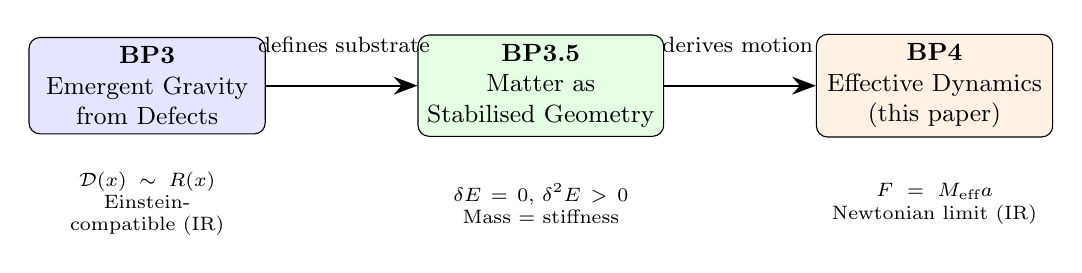
\begin{tikzpicture}[
    box/.style={draw, rounded corners, minimum width=3cm, minimum height=1.2cm, align=center, font=\small},
    arrow/.style={-{Stealth[length=3mm]}, thick}
]
    % BP3 box
    \node[box, fill=blue!10] (bp3) at (0,0) {\textbf{BP3}\\Emergent Gravity\\from Defects};

    % BP3.5 box
    \node[box, fill=green!10] (bp35) at (5,0) {\textbf{BP3.5}\\Matter as\\Stabilised Geometry};

    % BP4 box
    \node[box, fill=orange!10] (bp4) at (10,0) {\textbf{BP4}\\Effective Dynamics\\(this paper)};

    % Arrows
    \draw[arrow] (bp3) -- (bp35);
    \draw[arrow] (bp35) -- (bp4);

    % Labels
    \node[font=\footnotesize, above] at (2.5,0.3) {defines substrate};
    \node[font=\footnotesize, above] at (7.5,0.3) {derives motion};

    % Key contributions below
    \node[font=\scriptsize, text width=2.8cm, align=center] at (0,-1.5) {$\mathcal{D}(x) \sim R(x)$\\Einstein-compatible (IR)};
    \node[font=\scriptsize, text width=2.8cm, align=center] at (5,-1.5) {$\delta E = 0$, $\delta^2 E > 0$\\Mass = stiffness};
    \node[font=\scriptsize, text width=2.8cm, align=center] at (10,-1.5) {$F = \Meff a$\\Newtonian limit (IR)};
\end{tikzpicture}
\caption{Schematic: Progression through the Bridge Papers. BP3 establishes emergent gravity; BP3.5 defines matter as stabilised geometry; BP4 derives effective dynamics.}
\label{fig:progression}
\end{figure}

%==============================================================================
\section{Geometric Energy Functional}
%==============================================================================

\subsection{Units and Conventions}

Throughout this paper, we work in natural units where $\hbar = 1$, but retain $c$ explicitly to track mass-energy relations. When taking the Newtonian limit, we restore all factors of $c$. The metric signature is $(-,+,+,+)$.

\begin{assumption}[Substrate Structure]
The geometric substrate is characterised by a metric $g_{\mu\nu}$, with possible additional structure (torsion $T$, non-metricity $Q$). The substrate admits localised configurations that deviate from a flat background.
\end{assumption}

\begin{assumption}[Stabilisation Regime]
We consider configurations well within the stabilisation regime: the geometric energy functional has well-defined local minima, and perturbations remain small compared to barrier heights.
\end{assumption}

\begin{assumption}[Weak-Field, Infrared Limit]
For gravitational effects, we work in the weak-field, slow-motion regime where velocities satisfy $v \ll c$ and gravitational potentials satisfy $|\Phi| \ll c^2$. This is the regime where BP3 establishes Einstein-compatible dynamics.
\end{assumption}

\subsection{The Representative Functional}

We define a geometric energy functional of the form:
\begin{equation}
\label{eq:Egeom}
    \Egeom[g, \Phi, T, \ldots] = \int_\Omega \mathcal{L}(R, \Phi, \nabla\Phi, T, \ldots) \, \dd\mu_g,
\end{equation}
where $\Omega$ is the support of the configuration, $R$ denotes curvature invariants, $\Phi$ is the stabilisation order parameter, and $\dd\mu_g = \sqrt{|g|} \, \dd^4 x$ is the covariant volume element.

For concreteness, we consider a representative Lagrangian density:
\begin{equation}
\label{eq:Lagrangian}
    \mathcal{L} = \frac{c^4}{16\pi \Geff}\left( R + \alpha_1 \ell^2 R^2 + \alpha_2 \ell^2 R_{\mu\nu}R^{\mu\nu} \right) + \frac{1}{2}c^2 (\nabla \Phi)^2 + V(\Phi) + \beta \ell^2 T_{\mu\nu\rho}T^{\mu\nu\rho},
\end{equation}
where:
\begin{itemize}
    \item $\Geff$ is the effective gravitational coupling that emerges from the defect-curvature correspondence (BP3 shows $\Geff \to G$ in the infrared limit);
    \item $\ell$ is a characteristic length scale (related to the coherence scale $\ell_c$ of BP3);
    \item $\alpha_1, \alpha_2, \beta$ are dimensionless coupling constants;
    \item The $R^2$ and $R_{\mu\nu}R^{\mu\nu}$ terms encode higher-order defect contributions.
\end{itemize}

\begin{remark}[Class Representative---Independence from Specific Form]
The functional~\eqref{eq:Lagrangian} is a \emph{class representative}, not a final theory. \textbf{None of the results in Sections 4--7 depend on}:
\begin{itemize}
    \item the detailed form of the stabilising potential $V(\Phi)$;
    \item the numerical values of coefficients $\alpha_1$, $\alpha_2$, $\beta$ in $\mathcal{L}$;
    \item the specific profile shape of the stabilised configuration.
\end{itemize}
\textbf{The derivations require only}:
\begin{itemize}
    \item existence of a stable local minimum ($\delta\Egeom = 0$, $\delta^2\Egeom > 0$);
    \item a translational zero mode (broken translation symmetry);
    \item finite gradient energy ($\int |\nabla\Phi_0|^2 \, \dd^3x < \infty$).
\end{itemize}
The results are therefore generic to \emph{any class of stabilised geometric configurations} satisfying these structural requirements. Changing the Lagrangian within this class modifies quantitative coefficients (e.g., $\kappa$) but not the qualitative structure: mass from gradient energy, $F = \Meff a$, gravitational interaction via backreaction, and the proportionality of inertial and gravitational mass.
\end{remark}

\begin{remark}[Connection to BP3 Defect Density]
The curvature terms in~\eqref{eq:Lagrangian} encode the continuum limit of defect accumulation. In BP3, the defect density $\mathcal{D}(x)$ maps to scalar curvature as $\mathcal{D} \sim \alpha R$. The higher-derivative terms $R^2$, $R_{\mu\nu}R^{\mu\nu}$ capture corrections at scales approaching $\ell$, where the continuum approximation receives discrete corrections.
\end{remark}

\subsection{Stabilising Potential}

The potential $V(\Phi)$ is chosen to admit stable localised solutions. A representative form is:
\begin{equation}
\label{eq:potential}
    V(\Phi) = \frac{\lambda}{4}\left(\Phi^2 - v^2\right)^2,
\end{equation}
where $v$ is a vacuum expectation value and $\lambda > 0$ is a coupling constant with dimensions of energy per volume. This potential has minima at $\Phi = \pm v$ and supports domain-wall-like and solitonic solutions.

More generally, any potential satisfying:
\begin{enumerate}[label=(\roman*)]
    \item $V(\Phi) \geq 0$ with $V(\Phi_0) = 0$ at vacuum;
    \item $V''(\Phi_0) > 0$ ensuring stability;
    \item Appropriate boundary conditions at spatial infinity,
\end{enumerate}
will support stabilised configurations.

\begin{figure}[H]
\centering
\begin{tikzpicture}[scale=1.2, every node/.style={font=\small}]
    % Axes
    \draw[->] (-3,0) -- (3,0) node[right] {$\Phi$};
    \draw[->] (0,-0.3) -- (0,2.5) node[above] {$V$};
    % Potential curve
    \draw[thick, blue, domain=-2.5:2.5, samples=100] plot (\x, {0.3*(\x*\x - 2)*(\x*\x - 2)});
    % Minima
    \fill[red] (-1.414,0) circle (2pt) node[below] {$-v$};
    \fill[red] (1.414,0) circle (2pt) node[below] {$+v$};
    % Barrier
    \fill[black] (0,1.2) circle (1.5pt);
\end{tikzpicture}
\caption{Schematic: Double-well potential $V(\Phi) = \frac{\lambda}{4}(\Phi^2 - v^2)^2$ with stable minima at $\pm v$. The barrier height determines stability against large perturbations.}
\label{fig:stabilising-potential}
\end{figure}

%==============================================================================
\section{Stabilised Geometric Configurations}
%==============================================================================

\subsection{Existence of Localised Solutions}

We seek localised, static solutions $\Phi_0(\mathbf{x})$ to the field equations derived from~\eqref{eq:Egeom}. In the limit where gravitational backreaction is neglected (probe limit on a flat background), the field equation for $\Phi$ reduces to:
\begin{equation}
\label{eq:field_eq}
    c^2 \nabla^2 \Phi = V'(\Phi).
\end{equation}

For the potential~\eqref{eq:potential}, this admits the kink solution in one dimension:
\begin{equation}
\label{eq:kink}
    \Phi_0(x) = v \tanh\left(\frac{x}{\xi}\right), \qquad \xi = \sqrt{\frac{2c^2}{\lambda v^2}},
\end{equation}
where $\xi$ is the characteristic width of the configuration---the geometric scale over which the stabilised structure is localised.

In three dimensions, spherically symmetric solutions (hedgehog configurations) exist for appropriate field content. The general structure is:
\begin{equation}
\label{eq:3d_profile}
    \Phi_0(\mathbf{x}) = f(r) \hat{\mathbf{n}}(\theta, \phi),
\end{equation}
where $f(r)$ is a radial profile function satisfying appropriate boundary conditions: $f(0) = 0$ (regularity at origin), $f(\infty) = v$ (approach to vacuum).

\subsection{Stabilisation Conditions}

A configuration $\Phi_0$ is stabilised if it satisfies:

\begin{proposition}[Stabilisation]
\label{prop:stabilisation}
Let $\Phi_0$ be a static solution of~\eqref{eq:field_eq}. Then $\Phi_0$ is stabilised if:
\begin{enumerate}[label=(\roman*)]
    \item $\delta \Egeom[\Phi_0] = 0$ (critical point), and
    \item $\delta^2 \Egeom[\Phi_0] > 0$ (local minimum).
\end{enumerate}
The second variation is given by:
\begin{equation}
\label{eq:second_var}
    \delta^2 \Egeom = \int \dd^3 x \, \eta \left( -c^2\nabla^2 + V''(\Phi_0) \right) \eta,
\end{equation}
where $\eta$ is a perturbation. Positivity requires the operator $\mathcal{O} = -c^2\nabla^2 + V''(\Phi_0)$ to have no negative eigenvalues (excluding zero modes associated with symmetries).
\end{proposition}

For the kink solution~\eqref{eq:kink}, the operator $\mathcal{O}$ has a zero mode corresponding to translational invariance but no negative modes, confirming stability.

\subsection{Classification of Stabilisation Mechanisms}

Following BP3.5, stabilisation can arise from three mechanisms:

\textbf{Curvature Trapping}: The configuration occupies a local minimum of $\Egeom$ separated from lower-energy states by potential barriers. This is the mechanism operative for the kink solution.

\textbf{Torsional Closure}: If the substrate admits torsion, closed torsion loops can provide topological stabilisation. The closure condition:
\begin{equation}
    \oint_C \Gamma^\lambda_{\mu\nu} \, \dd x^\mu = 2\pi n,
\end{equation}
for integer $n$, constrains the configuration.

\textbf{Topological Persistence}: Configurations with non-trivial homotopy classes (e.g., $\pi_3(S^2) = \mathbb{Z}$ for hedgehogs) cannot be continuously deformed to the vacuum. The topological charge:
\begin{equation}
    Q = \frac{1}{4\pi} \int \dd^3 x \, \epsilon^{ijk} \hat{\Phi} \cdot (\partial_i \hat{\Phi} \times \partial_j \hat{\Phi}),
\end{equation}
is conserved under continuous evolution.

\begin{figure}[H]
\centering
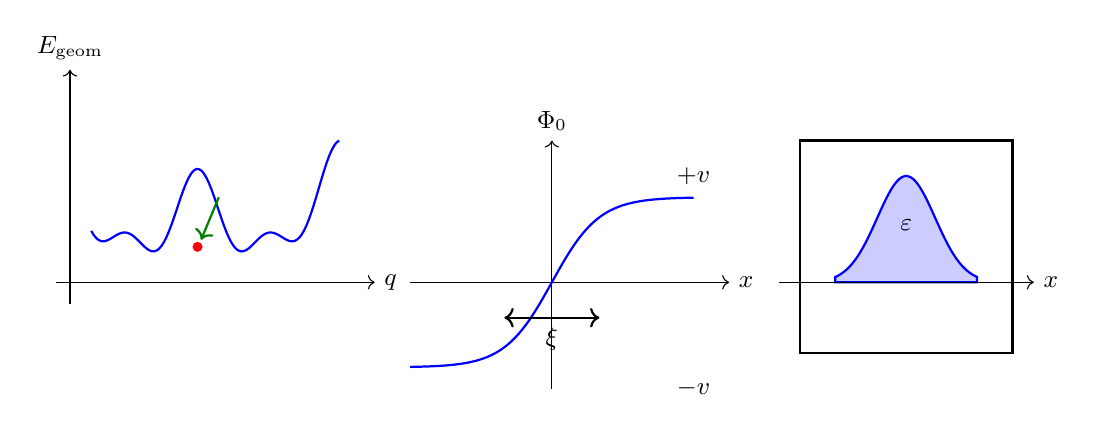
\begin{tikzpicture}[scale=0.9, every node/.style={font=\small}]
    % Energy landscape
    \begin{scope}[shift={(-5,0)}]
        \draw[->] (-2,0) -- (2.5,0) node[right] {$q$};
        \draw[->] (-1.8,-0.3) -- (-1.8,3) node[above] {$\Egeom$};
        \draw[thick, blue, domain=-1.5:2, samples=100]
            plot (\x, {0.8 + 0.5*cos(180*\x) + 0.3*cos(360*\x) + 0.1*\x*\x});
        \fill[red] (0,0.5) circle (2pt);
        \draw[->, thick, green!50!black] (0.3,1.2) -- (0.05,0.6);
    \end{scope}

    % Stabilised configuration profile
    \begin{scope}[shift={(0,0)}]
        \draw[->] (-2,0) -- (2.5,0) node[right] {$x$};
        \draw[->] (0,-1.5) -- (0,2) node[above] {$\Phi_0$};
        \draw[thick, blue, domain=-2:2, samples=100] plot (\x, {1.2*tanh(1.5*\x)});
        \node at (2,1.5) {$+v$};
        \node at (2,-1.5) {$-v$};
        \draw[<->, thick] (-0.67,-0.5) -- (0.67,-0.5) node[midway, below] {$\xi$};
    \end{scope}

    % Rest energy
    \begin{scope}[shift={(5,0)}]
        \draw[thick] (-1.5,-1) rectangle (1.5,2);
        \draw[thick, blue, fill=blue!20] plot[smooth, domain=-1:1, samples=50]
            (\x, {1.5*exp(-3*\x*\x)}) -- (1,0) -- (-1,0) -- cycle;
        \node at (0,0.8) {$\varepsilon$};
        \draw[->] (-1.8,0) -- (1.8,0) node[right] {$x$};
    \end{scope}
\end{tikzpicture}
\caption{Schematic: Left: Energy landscape over configuration parameter $q$; the red dot marks a stable minimum. Centre: Kink profile $\Phi_0(x)$ with width $\xi$. Right: Energy density $\varepsilon(\mathbf{x})$ whose integral gives rest energy $E_0$.}
\label{fig:stabilised}
\end{figure}

\subsection{Rest Energy of Stabilised Configurations}

The rest energy of a stabilised configuration is the value of the geometric energy functional at the minimum:
\begin{equation}
\label{eq:rest_energy}
    E_0 = \Egeom[\Phi_0] = \int \dd^3 x \left[ \frac{1}{2}c^2|\nabla \Phi_0|^2 + V(\Phi_0) \right].
\end{equation}

For the kink solution~\eqref{eq:kink} in one spatial dimension, dimensional analysis combined with the explicit integral yields the scaling form:
\begin{equation}
    E_0^{\text{(kink)}} = C_{\text{kink}} \cdot v^2 \xi \cdot A, \qquad C_{\text{kink}} = \frac{4}{3},
\end{equation}
where $A$ is the transverse area, $v$ is the field amplitude scale, and $\xi = \sqrt{2c^2/(\lambda v^2)}$ is the characteristic width. The numerical prefactor $C_{\text{kink}} = 4/3$ is specific to the $\tanh$ profile; different profile shapes within the same potential class yield order-unity prefactors.

More generally, for any localised configuration stabilised by a potential with scale $\lambda$ and amplitude $v$:
\begin{equation}
    E_0 \sim v^2 \xi \cdot A \sim \frac{c v^3}{\sqrt{\lambda}},
\end{equation}
up to an order-one numerical constant depending on profile choice. The dependence on $v$ (field amplitude), $\lambda$ (coupling/stiffness), and spatial extent is fixed by dimensional analysis; only the numerical prefactor requires explicit calculation.

This rest energy is the geometric origin of mass: a stabilised configuration carries an irreducible energy content $E_0$ that persists even at rest.

%==============================================================================
\section{Collective Coordinate Dynamics}
%==============================================================================

This section contains the core derivation of the paper: the emergence of Newtonian dynamics from collective-coordinate motion of stabilised geometric configurations.

\subsection{Promoting Translation to a Collective Coordinate}

Consider a stabilised configuration $\Phi_0(\mathbf{x})$ centred at the origin. We now allow the centre to move:
\begin{equation}
\label{eq:collective}
    \Phi(\mathbf{x}, t) = \Phi_0(\mathbf{x} - \mathbf{X}(t)),
\end{equation}
where $\mathbf{X}(t)$ is the collective coordinate representing the position of the configuration's centre.

The ansatz~\eqref{eq:collective} assumes the configuration maintains its shape during motion---the \emph{rigid body approximation}. This is valid when:
\begin{enumerate}[label=(\roman*)]
    \item Velocities are small compared to internal relaxation rates: $|\dot{\mathbf{X}}| \ll c$;
    \item External perturbations are weak compared to the stabilisation energy.
\end{enumerate}

Under these conditions, the full field dynamics reduce to the dynamics of the collective coordinate $\mathbf{X}(t)$.

\subsection{Derivation of the Effective Lagrangian}

We substitute the ansatz~\eqref{eq:collective} into the action:
\begin{equation}
    S = \int \dd t \int \dd^3 x \, \mathcal{L}[\Phi, \partial_\mu \Phi].
\end{equation}

The time derivative of $\Phi$ is:
\begin{equation}
    \partial_t \Phi = -\dot{X}^i \partial_i \Phi_0(\mathbf{x} - \mathbf{X}).
\end{equation}

The kinetic term in the Lagrangian density contributes:
\begin{equation}
    \frac{1}{2c^2}(\partial_t \Phi)^2 = \frac{1}{2c^2} \dot{X}^i \dot{X}^j \, \partial_i\Phi_0 \, \partial_j\Phi_0.
\end{equation}

For an \emph{isotropic} configuration, the tensor $\int \partial_i\Phi_0 \, \partial_j\Phi_0 \, \dd^3x$ is proportional to $\delta_{ij}$:
\begin{equation}
    \int \dd^3 x \, \partial_i\Phi_0 \, \partial_j\Phi_0 = \frac{1}{3}\delta_{ij} \int \dd^3 x \, |\nabla\Phi_0|^2.
\end{equation}

Integrating over space, the kinetic contribution to the Lagrangian becomes:
\begin{equation}
\label{eq:kinetic_int}
    \int \dd^3 x \, \frac{1}{2c^2}(\partial_t \Phi)^2 = \frac{1}{2} \cdot \frac{|\dot{\mathbf{X}}|^2}{c^2} \cdot \frac{1}{3} \int \dd^3 x \, |\nabla \Phi_0|^2.
\end{equation}

The potential term is independent of $\dot{\mathbf{X}}$:
\begin{equation}
    \int \dd^3 x \, V(\Phi_0(\mathbf{x} - \mathbf{X})) = \int \dd^3 x' \, V(\Phi_0(\mathbf{x}')) = E_V,
\end{equation}
which is constant (the potential energy of the static configuration).

We define the \textbf{effective inertial mass}. For an isotropic configuration, the isotropy average yields:
\begin{equation}
\label{eq:Meff}
    \boxed{\Meff \equiv \frac{1}{3c^2} \int \dd^3 x \, |\nabla \Phi_0(\mathbf{x})|^2}
\end{equation}

\textbf{Origin of the $1/3$ factor}: For an isotropic configuration, the tensor $\int \partial_i\Phi_0 \partial_j\Phi_0 \, \dd^3x = \frac{1}{3}\delta_{ij}\int|\nabla\Phi_0|^2\,\dd^3x$ by rotational symmetry. This factor is \emph{not} absorbed into other definitions---it is an intrinsic consequence of isotropy and appears explicitly in $\Meff$.

\textbf{Dimensional check}: $[\nabla\Phi_0]^2$ has dimensions of $[\text{energy/volume}]$ (from the gradient energy density), so $\int|\nabla\Phi_0|^2\,\dd^3x$ has dimensions $[\text{energy}]$. Division by $c^2$ yields $[\text{mass}]$.

For non-isotropic configurations, the effective mass becomes a tensor $M_{ij}^{\text{eff}}$, and the scalar $\Meff$ should be understood as the directionally averaged value.

Thus, the effective Lagrangian is:
\begin{equation}
\label{eq:Leff}
    \boxed{\Leff = -E_0 + \frac{1}{2}\Meff |\dot{\mathbf{X}}|^2 + \order{\dot{X}^4/c^4}}
\end{equation}

This is the standard non-relativistic Lagrangian for a point particle with mass $\Meff$ and rest energy $E_0$.

\begin{remark}[Mass from Gradient Energy]
The effective mass~\eqref{eq:Meff} arises from the gradient energy of the static configuration. This is the geometric manifestation of inertia: the resistance to \emph{time-dependent translation} of stabilised geometry. Configurations with steeper gradients (more tightly wound geometry) have greater effective mass because more geometric structure must be translated in time. This is distinct from elastic stiffness (resistance to static deformation)---inertia here specifically characterises the dynamical response to acceleration. The mass is determined entirely by the static solution $\Phi_0$---no additional input is required.
\end{remark}

\subsection{Relation Between Effective Mass and Rest Energy}

For configurations stabilised by the potential~\eqref{eq:potential}, the virial theorem relates gradient and potential energies. From the scaling properties of the field equation, one can show:
\begin{equation}
    \int \dd^3x \, \frac{1}{2}c^2|\nabla\Phi_0|^2 = \int \dd^3x \, V(\Phi_0) \quad \text{(equipartition)}.
\end{equation}

Under equipartition, the rest energy is:
\begin{equation}
    E_0 = 2 \int \dd^3x \, \frac{1}{2}c^2|\nabla\Phi_0|^2 = c^2 \int \dd^3x \, |\nabla\Phi_0|^2.
\end{equation}

Comparing with~\eqref{eq:Meff}:
\begin{equation}
\label{eq:mass_energy}
    \Meff = \frac{1}{3c^2} \cdot \frac{E_0}{c^2} \cdot c^2 = \frac{E_0}{3c^2} \quad \text{(equipartition, isotropic)}.
\end{equation}

More generally:
\begin{equation}
\label{eq:mass_energy_general}
    \Meff = \kappa \frac{E_0}{c^2},
\end{equation}
where $\kappa$ is a dimensionless \emph{geometric factor} of order unity that depends on:
\begin{itemize}
    \item The shape of the configuration (isotropy gives $\kappa = 1/3$ times the gradient/total energy ratio);
    \item The specific form of the stabilising potential;
    \item Whether equipartition holds.
\end{itemize}
\textbf{Important}: The factor $\kappa$ is \emph{not assumed} to be identical for all configurations. Different stabilisation classes may yield different values of $\kappa$. Universality of $\kappa$ emerges only under specific symmetry/equipartition conditions (Section~7).

\begin{proposition}[Mass-Energy Correspondence]
\label{prop:mass-energy}
The effective inertial mass $\Meff$ is proportional to the rest energy $E_0$ of the stabilised configuration:
\begin{equation}
    \Meff = \kappa \frac{E_0}{c^2},
\end{equation}
where $\kappa$ is determined by the geometric structure of the solution. For families of configurations sharing the same stabilisation structure (same potential class, same equipartition properties), $\kappa$ is constant.
\end{proposition}

Unlike the Standard Model, where inertial mass enters as a parameter (via the Higgs mechanism or explicit mass terms), here inertia is \emph{computed} from the stabilised geometric configuration. The mass is not an input---it is a derived consequence of the configuration's gradient structure.

\subsection{Momentum and Equation of Motion}

From the effective Lagrangian~\eqref{eq:Leff}, the canonical momentum is:
\begin{equation}
\label{eq:momentum}
    \mathbf{P} = \frac{\partial \Leff}{\partial \dot{\mathbf{X}}} = \Meff \dot{\mathbf{X}}.
\end{equation}

This is the standard momentum-velocity relation with effective mass $\Meff$.

The Euler-Lagrange equation gives:
\begin{equation}
\label{eq:EoM_free}
    \frac{\dd}{\dd t}\left( \Meff \dot{\mathbf{X}} \right) = 0 \quad \Rightarrow \quad \Meff \ddot{\mathbf{X}} = 0.
\end{equation}

In the absence of external influences, the configuration moves at constant velocity---Newton's first law emerges automatically from the collective-coordinate dynamics.

\subsection{Including External Perturbations}

Now consider a spatially varying perturbation $U(\mathbf{x})$ to the background geometry. This could arise from:
\begin{itemize}
    \item Another stabilised configuration (gravitational interaction);
    \item An external geometric distortion;
    \item Boundary effects.
\end{itemize}

The perturbation modifies the energy functional:
\begin{equation}
    \Egeom[\Phi; U] = \int \dd^3 x \left[ \frac{1}{2}c^2|\nabla \Phi|^2 + V(\Phi) + U(\mathbf{x}) \varepsilon_\Phi(\mathbf{x}) \right],
\end{equation}
where $\varepsilon_\Phi(\mathbf{x})$ is the energy density of the configuration.

For the collective coordinate ansatz, assuming $U$ varies slowly on the scale $\xi$:
\begin{equation}
    \int \dd^3 x \, U(\mathbf{x}) \varepsilon_\Phi(\mathbf{x} - \mathbf{X}) \approx U(\mathbf{X}) \int \dd^3 x' \, \varepsilon_\Phi(\mathbf{x}') = U(\mathbf{X}) E_0.
\end{equation}

The effective Lagrangian becomes:
\begin{equation}
\label{eq:Leff_ext}
    \Leff = -E_0 + \frac{1}{2}\Meff |\dot{\mathbf{X}}|^2 - U(\mathbf{X}) E_0.
\end{equation}

The equation of motion is now:
\begin{equation}
\label{eq:Newton}
    \boxed{\Meff \ddot{\mathbf{X}} = -E_0 \nabla U(\mathbf{X}) \equiv \mathbf{F}}
\end{equation}

This recovers Newton's second law: $\mathbf{F} = \Meff \mathbf{a}$ with force $\mathbf{F} = -E_0 \nabla U$.

\begin{figure}[H]
\centering
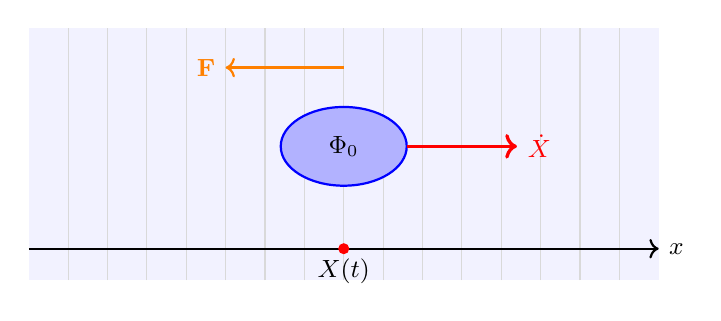
\begin{tikzpicture}[scale=1.0, every node/.style={font=\small}]
    % Background
    \fill[blue!5] (-4,-1.2) rectangle (4,2);
    \foreach \x in {-3.5,-3,...,3.5} {
        \draw[gray!30, thin] (\x,-1.2) -- (\x,2);
    }
    % Configuration
    \draw[thick, blue, fill=blue!30] (0,0.5) ellipse (0.8 and 0.5);
    \node at (0,0.5) {$\Phi_0$};
    % Position axis
    \draw[->, thick] (-4,-0.8) -- (4,-0.8) node[right] {$x$};
    \fill[red] (0,-0.8) circle (2pt);
    \node[below] at (0,-0.8) {$X(t)$};
    % Velocity arrow
    \draw[->, very thick, red] (0.8,0.5) -- (2.2,0.5) node[right] {$\dot{X}$};
    % Force arrow
    \draw[thick, orange, ->] (0,1.5) -- (-1.5,1.5) node[left] {$\mathbf{F}$};
\end{tikzpicture}
\caption{Schematic: Collective coordinate dynamics. The configuration $\Phi_0$ moves rigidly with centre position $X(t)$ and velocity $\dot{X}$. External perturbations produce force $\mathbf{F}$, yielding $\Meff \ddot{X} = F$.}
\label{fig:collective}
\end{figure}

\subsection{The Newtonian Limit: $F = \Meff a$}

Equation~\eqref{eq:Newton} has the form of Newton's second law. For a gravitational perturbation $U = \PhiG/c^2$ (dimensionless gravitational potential), the force becomes:
\begin{equation}
    \mathbf{F} = -\frac{E_0}{c^2} \nabla \PhiG = -\Mgrav \nabla \PhiG,
\end{equation}
where we identify the \textbf{gravitational mass}:
\begin{equation}
\label{eq:Mgrav}
    \boxed{\Mgrav \equiv \frac{E_0}{c^2}}
\end{equation}

The equation of motion becomes:
\begin{equation}
    \Meff \ddot{\mathbf{X}} = -\Mgrav \nabla\PhiG.
\end{equation}

Using~\eqref{eq:mass_energy_general}:
\begin{equation}
\label{eq:ratio}
    \frac{\Mgrav}{\Meff} = \frac{E_0/c^2}{\kappa E_0/c^2} = \frac{1}{\kappa}.
\end{equation}

For a free-falling trajectory in a gravitational field:
\begin{equation}
    \ddot{\mathbf{X}} = -\frac{1}{\kappa} \nabla\PhiG.
\end{equation}

\begin{remark}[Universality Conditions]
The ratio $\Mgrav/\Meff = 1/\kappa$ is constant for configurations belonging to the same stabilisation class (same $\kappa$). \textbf{Universality}---the statement that all matter falls at the same rate---emerges \emph{only when} the following conditions are satisfied:
\begin{enumerate}[label=(\alph*)]
    \item All configurations belong to the same potential class (same $V(\Phi)$ structure);
    \item The virial/equipartition condition holds for all configurations;
    \item Isotropy is satisfied (or directional averaging is appropriate).
\end{enumerate}
This is not guaranteed \emph{a priori} but is a consequence of the stabilisation structure. For the representative potential~\eqref{eq:potential} with equipartition and isotropy, $\kappa = 1/3$ for all configurations in the class. Violations of any condition would produce composition-dependent free-fall, subject to empirical test (Section~8.2).
\end{remark}

%==============================================================================
\section{Interaction Between Stabilised Configurations}
%==============================================================================

The interaction between stabilised configurations is not introduced as a separate postulate; it emerges from the geometric energy functional itself. A configuration of non-trivial geometry perturbs its surroundings, and another configuration responds to this perturbation through the same energy functional that determines its inertia. This section derives how the Newtonian gravitational interaction arises from this geometric logic.

\begin{center}
\fbox{\parbox{0.9\textwidth}{
\textbf{Dependence on BP3}: All gravitational dynamics invoked in this section are \emph{inherited from BP3}. BP4 does not independently assume Einstein gravity; it works entirely within the emergent framework established there. The field equations~\eqref{eq:Einstein_IR} below are \emph{derived consequences} of the BP3 defect-curvature correspondence, valid in the infrared limit.
}}
\end{center}

\subsection{Geometric Backreaction: From Functional Variation to Field Equations}

A stabilised configuration is not merely a passive entity embedded in geometry---it \emph{is} a configuration of the geometry. As such, it perturbs the surrounding substrate.

To derive the gravitational interaction, we return to the geometric energy functional~\eqref{eq:Egeom} and consider the response of the metric to the presence of a localised energy density.

Consider a configuration $\Phi_A$ centred at position $\mathbf{X}_A$. The associated stress-energy tensor is:
\begin{equation}
    T_{\mu\nu}^{(A)} = c^2 \partial_\mu\Phi_A \partial_\nu\Phi_A - g_{\mu\nu}\left[\frac{c^2}{2}(\partial\Phi_A)^2 + V(\Phi_A)\right].
\end{equation}

\emph{This object has the same algebraic form as a scalar-field stress-energy tensor, but here it is a derived effective quantity encoding geometric energy density, not a fundamental quantum field.} It encodes how the geometric energy of the stabilised configuration couples to the metric.

In the rest frame of a static configuration: $T_{00}^{(A)} = \varepsilon_A$, the energy density.

Varying the geometric part of the action~\eqref{eq:Lagrangian} with respect to the metric yields field equations. In the infrared limit where BP3 establishes Einstein-compatible dynamics, these reduce to:
\begin{equation}
\label{eq:Einstein_IR}
    G_{\mu\nu} + \Lambda_{\text{eff}} g_{\mu\nu} = \frac{8\pi\Geff}{c^4} T_{\mu\nu},
\end{equation}
where $\Geff \to G$ (Newton's constant) in the infrared and $\Lambda_{\text{eff}}$ includes any cosmological contribution from the defect background.

\begin{remark}[Higher-Order Corrections]
At scales approaching $\ell$ or in strong-field regimes, the $R^2$ and $R_{\mu\nu}R^{\mu\nu}$ corrections in~\eqref{eq:Lagrangian} become significant and modify~\eqref{eq:Einstein_IR}. The present analysis applies in the infrared limit where these corrections are negligible.
\end{remark}

\subsection{Linearised Response and Perturbation Propagation}

The linearised field equations below are \emph{derived consequences} of the effective geometric dynamics, not postulated starting points. They arise from variation of the geometric functional~\eqref{eq:Egeom} in the infrared limit, as established in BP3. The standard Newtonian potential emerges as an effective description valid at scales $r \gg \ell$.

In the weak-field limit, we write $g_{\mu\nu} = \eta_{\mu\nu} + h_{\mu\nu}$ with $|h_{\mu\nu}| \ll 1$. Linearising~\eqref{eq:Einstein_IR}:
\begin{equation}
\label{eq:linearised}
    \Box \bar{h}_{\mu\nu} = -\frac{16\pi\Geff}{c^4} T_{\mu\nu}^{(A)},
\end{equation}
where $\bar{h}_{\mu\nu} = h_{\mu\nu} - \frac{1}{2}\eta_{\mu\nu}h$ is the trace-reversed perturbation.

The retarded Green's function solution is:
\begin{equation}
    h_{\mu\nu}(\mathbf{x}, t) = \frac{4\Geff}{c^4} \int \dd^3 x' \, \frac{T_{\mu\nu}^{(A)}(\mathbf{x}', t_{\text{ret}})}{|\mathbf{x} - \mathbf{x}'|},
\end{equation}
where $t_{\text{ret}} = t - |\mathbf{x} - \mathbf{x}'|/c$.

In the \textbf{static or slow-motion limit}, this reduces to:
\begin{equation}
    h_{00}(\mathbf{x}) \approx -\frac{2\PhiG^{(A)}(\mathbf{x})}{c^2},
\end{equation}
where the gravitational potential from configuration $A$ is:
\begin{equation}
\label{eq:Phi_A}
    \PhiG^{(A)}(\mathbf{x}) = -\Geff \int \dd^3 x' \, \frac{\varepsilon_A(\mathbf{x}')}{c^2 |\mathbf{x} - \mathbf{x}'|} = -\Geff \int \dd^3 x' \, \frac{\rho_A(\mathbf{x}')}{|\mathbf{x} - \mathbf{x}'|},
\end{equation}
with $\rho_A = \varepsilon_A/c^2$ the mass density.

For a \textbf{localised configuration} with total energy $E_A$ and characteristic size $\xi \ll r$:
\begin{equation}
\label{eq:Newtonian_pot}
    \PhiG^{(A)}(\mathbf{x}) \approx -\frac{\Geff M_A}{|\mathbf{x} - \mathbf{X}_A|}, \qquad M_A = \frac{E_A}{c^2}.
\end{equation}

This is the Newtonian gravitational potential, recovered from the geometric backreaction of a stabilised configuration.

\subsection{Response of a Second Configuration}

Now consider a second configuration $\Phi_B$ at position $\mathbf{X}_B$. It experiences the perturbation from $A$ through the modified effective Lagrangian:
\begin{equation}
    \Leff^{(B)} = -E_B + \frac{1}{2}M_B^{\text{eff}} |\dot{\mathbf{X}}_B|^2 - M_B^{\text{grav}} \PhiG^{(A)}(\mathbf{X}_B).
\end{equation}

Using~\eqref{eq:Newtonian_pot} and $M_B^{\text{grav}} = E_B/c^2$:
\begin{equation}
    \Leff^{(B)} = -E_B + \frac{1}{2}M_B^{\text{eff}} |\dot{\mathbf{X}}_B|^2 + \frac{\Geff M_A^{\text{grav}} M_B^{\text{grav}}}{|\mathbf{X}_B - \mathbf{X}_A|}.
\end{equation}

The equation of motion for $B$ is:
\begin{equation}
\label{eq:two_body}
    M_B^{\text{eff}} \ddot{\mathbf{X}}_B = -\frac{\Geff M_A^{\text{grav}} M_B^{\text{grav}}}{|\mathbf{X}_B - \mathbf{X}_A|^2} \hat{\mathbf{r}}_{AB},
\end{equation}
where $\hat{\mathbf{r}}_{AB}$ points from $A$ to $B$.

Using $M^{\text{eff}} = \kappa M^{\text{grav}}$ for both configurations (same stabilisation class):
\begin{equation}
    \ddot{\mathbf{X}}_B = -\frac{\Geff M_A^{\text{grav}}}{\kappa |\mathbf{X}_B - \mathbf{X}_A|^2} \hat{\mathbf{r}}_{AB}.
\end{equation}

This recovers Newton's law of gravitation (with effective coupling $\Geff/\kappa$) from the geometric interaction of stabilised configurations.

\begin{figure}[H]
\centering
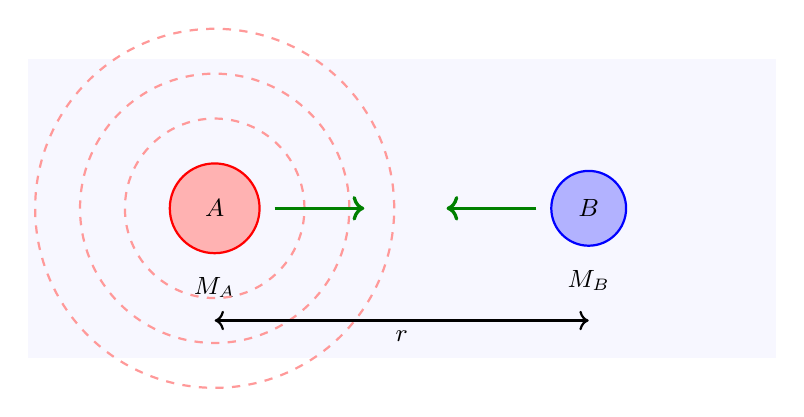
\begin{tikzpicture}[scale=0.95, every node/.style={font=\small}]
    % Background
    \fill[blue!3] (-5,-1.5) rectangle (5,2.5);
    % Configuration A
    \draw[thick, red, fill=red!30] (-2.5,0.5) circle (0.6);
    \node at (-2.5,0.5) {$A$};
    \node[below] at (-2.5,-0.3) {$M_A$};
    % Configuration B
    \draw[thick, blue, fill=blue!30] (2.5,0.5) circle (0.5);
    \node at (2.5,0.5) {$B$};
    \node[below] at (2.5,-0.2) {$M_B$};
    % Perturbation waves
    \foreach \r in {1.2, 1.8, 2.4} {
        \draw[red!40, thick, dashed] (-2.5,0.5) circle (\r);
    }
    % Force arrows
    \draw[->, very thick, green!50!black] (-1.7,0.5) -- (-0.5,0.5);
    \draw[->, very thick, green!50!black] (1.8,0.5) -- (0.6,0.5);
    % Distance
    \draw[<->, thick] (-2.5,-1) -- (2.5,-1) node[midway, below] {$r$};
\end{tikzpicture}
\caption{Schematic: Two-body gravitational interaction. Configuration $A$ perturbs the geometry (dashed circles); $B$ responds to this perturbation. The inverse-square law $F \propto \Geff M_A M_B / r^2$ emerges in the IR limit.}
\label{fig:interaction}
\end{figure}

\subsection{Momentum Exchange and Conservation}

In a two-body system, conservation of total momentum follows from translational invariance of the total Lagrangian. The total momentum:
\begin{equation}
    \mathbf{P}_{\text{tot}} = M_A^{\text{eff}} \dot{\mathbf{X}}_A + M_B^{\text{eff}} \dot{\mathbf{X}}_B,
\end{equation}
is conserved: $\dot{\mathbf{P}}_{\text{tot}} = 0$.

This follows from Newton's third law, which holds because the interaction depends only on the separation $|\mathbf{X}_B - \mathbf{X}_A|$:
\begin{equation}
    \mathbf{F}_{A \to B} = -\mathbf{F}_{B \to A}.
\end{equation}

The geometric framework thus reproduces momentum conservation as a consequence of spatial homogeneity of the substrate.

%==============================================================================
\section{Gravitational Limit}
%==============================================================================

\subsection{Effective Potential from Geometric Energy}

The gravitational potential generated by a stabilised configuration arises from its geometric energy density. For a collection of configurations $\{A_i\}$ with rest energies $\{E_i\}$ at positions $\{\mathbf{X}_i\}$, the total gravitational potential at point $\mathbf{x}$ is:
\begin{equation}
\label{eq:potential_sum}
    \PhiG(\mathbf{x}) = -\Geff \sum_i \frac{E_i/c^2}{|\mathbf{x} - \mathbf{X}_i|} = -\Geff \sum_i \frac{M_i^{\text{grav}}}{|\mathbf{x} - \mathbf{X}_i|}.
\end{equation}

In the continuum limit with geometric energy density $\rhogeom(\mathbf{x}) = \varepsilon(\mathbf{x})/c^2$:
\begin{equation}
\label{eq:potential_int}
    \PhiG(\mathbf{x}) = -\Geff \int \dd^3 x' \, \frac{\rhogeom(\mathbf{x}')}{|\mathbf{x} - \mathbf{x}'|}.
\end{equation}

\subsection{Weak-Field Approximation and Poisson Equation}

The potential~\eqref{eq:potential_int} satisfies the Poisson equation:
\begin{equation}
\label{eq:Poisson}
    \boxed{\nabla^2 \PhiG = 4\pi \Geff \rhogeom}
\end{equation}

This is the standard result of Newtonian gravity, recovered from the effective dynamics of stabilised configurations in the infrared limit.

The key identification is:
\begin{equation}
\label{eq:rho_geom}
    \rhogeom(\mathbf{x}) = \frac{\varepsilon(\mathbf{x})}{c^2} = \frac{1}{c^2}\left[ \frac{c^2}{2}|\nabla \Phi|^2 + V(\Phi) \right],
\end{equation}
where $\varepsilon$ is the geometric energy density from Section~3.

In the infrared limit, $\Geff \to G$ (Newton's constant), recovering standard Newtonian gravity.

\begin{figure}[H]
\centering
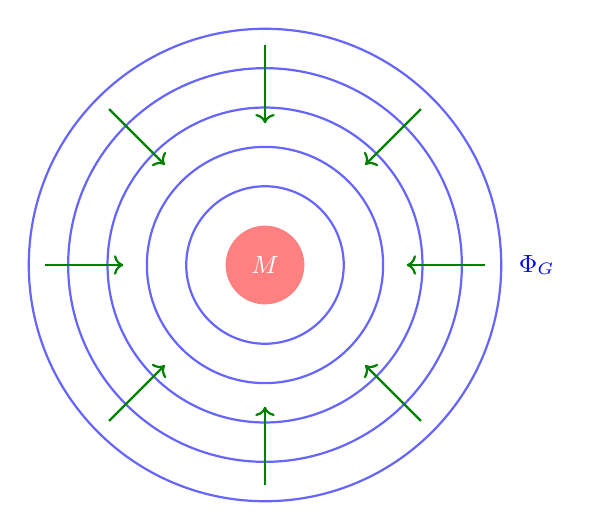
\begin{tikzpicture}[scale=1.0, every node/.style={font=\small}]
    % Central mass
    \fill[red!50] (0,0) circle (0.5);
    \node[white] at (0,0) {$M$};
    % Equipotential lines
    \foreach \r in {1, 1.5, 2, 2.5, 3} {
        \draw[blue!60, thick] (0,0) circle (\r);
    }
    % Field lines
    \foreach \angle in {0, 45, 90, 135, 180, 225, 270, 315} {
        \draw[->, thick, green!50!black] (\angle:2.8) -- (\angle:1.8);
    }
    % Label
    \node[right, blue] at (3.1,0) {$\PhiG$};
\end{tikzpicture}
\caption{Schematic: Gravitational potential $\PhiG = -\Geff M/r$ from a stabilised configuration. Equipotential surfaces (circles) and field lines (arrows) emerge from the Poisson equation in the IR limit.}
\label{fig:grav-potential}
\end{figure}

\subsection{Source Identification: No Separate Postulate}

The source of the gravitational field is the same geometric energy that determines inertial mass. No separate ``gravitational charge'' is introduced---the stress-energy tensor for a stabilised configuration is:
\begin{equation}
    T_{\mu\nu} = c^2\partial_\mu \Phi \partial_\nu \Phi - g_{\mu\nu} \left[ \frac{c^2}{2}(\partial \Phi)^2 + V(\Phi) \right].
\end{equation}

In the rest frame: $T_{00} = \varepsilon$, and:
\begin{equation}
    \Mgrav = \frac{1}{c^2}\int T_{00} \, \dd^3x = \frac{E_0}{c^2}.
\end{equation}

The absence of a separate sourcing postulate is a direct consequence of treating matter as geometry: the curvature content \emph{is} the source.

%==============================================================================
\section{Equivalence of Inertial and Gravitational Mass}
%==============================================================================

\subsection{Common Geometric Origin}

We have established:
\begin{enumerate}[label=(\roman*)]
    \item \textbf{Inertial mass} $\Meff$ arises from the gradient energy of the stabilised configuration (Eq.~\ref{eq:Meff}):
    \begin{equation}
        \Meff = \frac{1}{3c^2} \int \dd^3 x \, |\nabla \Phi_0|^2.
    \end{equation}

    \item \textbf{Rest energy} $E_0$ is the total geometric energy (Eq.~\ref{eq:rest_energy}):
    \begin{equation}
        E_0 = \int \dd^3 x \left[ \frac{c^2}{2}|\nabla \Phi_0|^2 + V(\Phi_0) \right].
    \end{equation}

    \item \textbf{Gravitational mass} $\Mgrav = E_0/c^2$ sources the gravitational field via the Poisson equation.
\end{enumerate}

Both masses are functionals of the same static solution $\Phi_0$, evaluated on the geometric energy functional $\Egeom$.

\subsection{Proportionality and Conditions for Universality}

From Proposition~\ref{prop:mass-energy}:
\begin{equation}
    \Meff = \kappa \Mgrav, \qquad \kappa = \frac{\int |\nabla\Phi_0|^2 \, \dd^3x}{3 E_0 / c^2}.
\end{equation}

The ratio $\Meff/\Mgrav = \kappa$ is:
\begin{itemize}
    \item \textbf{Determined by the solution}: Different configurations may have different $\kappa$.
    \item \textbf{Constant within a class}: Configurations sharing the same stabilisation structure (same potential class, same boundary conditions, same virial/equipartition properties) have the same $\kappa$.
\end{itemize}

\textbf{Universality emerges when}:
\begin{enumerate}[label=(\roman*)]
    \item All matter configurations belong to the same stabilisation class;
    \item The virial/equipartition condition $\int c^2|\nabla\Phi_0|^2/2 = \int V(\Phi_0)$ holds universally;
    \item Isotropy is satisfied (or the directional average is taken).
\end{enumerate}

Under these conditions, $\kappa$ becomes a universal constant, and the equivalence principle---equal acceleration in a gravitational field regardless of composition---follows.

\begin{proposition}[Geometric Basis for Equivalence]
\label{prop:equivalence}
The proportionality of inertial and gravitational mass follows from their common origin in the geometric energy functional. Universality of the proportionality constant $\kappa$ emerges for configurations satisfying common stabilisation/virial conditions. No additional postulate is required beyond the structure of $\Egeom$.
\end{proposition}

\begin{remark}[Limitations]
We do not claim to have proven that all matter satisfies the same virial condition. This is an \emph{assumption} about the universality of the stabilisation mechanism. Violations would manifest as composition-dependent free-fall acceleration---a prediction testable via equivalence principle experiments (see Section~8).
\end{remark}

%==============================================================================
\section{Predictions and Regime of Validity}
%==============================================================================

\subsection{Where the Framework Applies}

The derivations of this paper are valid in the following regime:
\begin{enumerate}[label=(\roman*)]
    \item \textbf{Stabilisation regime}: Configurations are at local minima of $\Egeom$ with $\delta^2 \Egeom > 0$.
    \item \textbf{Collective coordinate regime}: Internal relaxation is fast compared to centre-of-mass motion: $\omega_{\text{int}} \gg \omega_{\text{ext}}$.
    \item \textbf{Weak field}: $|\PhiG| \ll c^2$ so the linearised treatment applies.
    \item \textbf{Infrared limit}: Length scales $\gg \ell$ (the discrete/coherence scale) so $\Geff \approx G$.
    \item \textbf{Non-relativistic}: $|\dot{X}|^2 \ll c^2$ so higher-order terms in~\eqref{eq:Leff} are negligible.
\end{enumerate}

Standard Newtonian mechanics is recovered throughout this regime.

\subsection{Concrete Predictions and Potential Deviations}

The framework makes specific, falsifiable predictions for regimes where deviations from standard dynamics may occur:

\subsubsection{Prediction 1: Finite-Size Corrections to Gravity}

At distances $r \lesssim \xi$ (comparable to the configuration size), the $1/r$ potential receives corrections. From~\eqref{eq:Phi_A}, expanding for extended sources:
\begin{equation}
    \PhiG(r) = -\frac{\Geff M}{r}\left(1 + \frac{a_2}{r^2}\langle r'^2\rangle + \order{r^{-4}}\right),
\end{equation}
where $\langle r'^2\rangle \sim \xi^2$ is the mean-square radius of the configuration.

\textbf{Signature}: Deviation from inverse-square law at short range. For $\xi \sim 10^{-15}$~m (nuclear scale), deviations would appear below femtometer separations.

\subsubsection{Prediction 2: Composition-Dependent Free Fall}

If different matter types have different geometric factors $\kappa$, free-fall acceleration becomes composition-dependent:
\begin{equation}
    a = \frac{1}{\kappa}\nabla\PhiG.
\end{equation}

\textbf{Signature}: E\"otv\"os parameter $\eta = 2|a_1 - a_2|/(a_1 + a_2) \neq 0$.

Current bounds: $\eta < 10^{-14}$ (MICROSCOPE). Within our framework, universality of $\kappa$ is predicted for matter sharing the same stabilisation class. Violations would indicate multiple stabilisation mechanisms or breakdown of equipartition.

\subsubsection{Prediction 3: Higher-Derivative Corrections in Strong Fields}

The $R^2$ and $R_{\mu\nu}R^{\mu\nu}$ terms in~\eqref{eq:Lagrangian} produce corrections to the Newtonian potential:
\begin{equation}
    \PhiG(r) = -\frac{GM}{r}\left(1 + \frac{\alpha_{\text{eff}} \ell^2}{r^2} + \order{\ell^4/r^4}\right),
\end{equation}
where $\alpha_{\text{eff}}$ depends on $\alpha_1$, $\alpha_2$.

\textbf{Signature}: PPN-like corrections parametrised by $\ell$. For $\ell \sim \ell_{\text{Planck}}$, corrections are negligible at laboratory scales but may be relevant near black holes or in early-universe cosmology.

\subsubsection{Prediction 4: Velocity-Dependent Effective Mass Near Thresholds}

When configurations approach stabilisation thresholds (barriers comparable to kinetic energy), internal modes couple to translation. The effective mass acquires velocity dependence:
\begin{equation}
    \Meff(v) = \Meff^{(0)} + \delta M(v^2/c^2) + \order{v^4/c^4}.
\end{equation}

\textbf{Important clarification}: This velocity dependence is \emph{not} relativistic mass increase ($\gamma m$), which is a kinematic consequence of Lorentz invariance. Rather, it arises from \emph{internal mode coupling}---the collective-coordinate approximation breaks down when translational kinetic energy approaches the barrier height, and internal deformation modes become excited. The correction $\delta M$ depends on the second variation of $\Egeom$ around $\Phi_0$ and vanishes in the deep-stabilisation limit.

\textbf{Regime of validity}: This effect is relevant when $\frac{1}{2}\Meff v^2 \sim \Delta E_{\text{barrier}}$, i.e., for configurations near destabilisation thresholds. For deeply trapped configurations ($\Delta E_{\text{barrier}} \gg \frac{1}{2}\Meff c^2$), the velocity-dependent correction is negligible at non-relativistic speeds.

\textbf{Signature}: Anomalous inertia for highly excited configurations approaching destabilisation. This would manifest as composition-dependent inertial response in precision measurements.

\subsection{What BP5 Must Add}

This paper establishes classical effective dynamics. A complete treatment requires:
\begin{enumerate}[label=(\roman*)]
    \item \textbf{Quantum dynamics}: Superposition, interference, and tunnelling of stabilised configurations. The discreteness of stabilisation modes (Section~6 of BP3.5) suggests a natural quantisation, but deriving the full quantum mechanics is non-trivial.
    \item \textbf{Internal modes}: Excitation spectra and transitions between configurations. The vibrational modes around $\Phi_0$ define a spectrum that should connect to particle physics.
    \item \textbf{Relativistic extension}: Full Lorentz-covariant collective-coordinate dynamics, including spin and polarisation.
    \item \textbf{Multi-configuration effects}: Beyond two-body interactions---many-body correlations, statistical mechanics of configuration ensembles.
    \item \textbf{Coupling to gauge fields}: How electromagnetic and other interactions emerge from the geometric framework.
\end{enumerate}

These developments are deferred to BP5 and subsequent work.

\subsection{Explicit Domain of Validity}

For clarity, we summarise the regime where the present derivations apply:
\begin{itemize}
    \item \textbf{Applicable}: Weak gravitational fields ($|\PhiG| \ll c^2$); non-relativistic collective motion ($v \ll c$); isolated or weakly interacting stabilised configurations; length scales well above the coherence scale ($r \gg \ell$).
    \item \textbf{Not yet covered}: Relativistic velocities; quantum superposition of configurations; internal mode quantisation; strong-field gravitational dynamics; many-body correlations beyond pairwise interaction.
\end{itemize}
The results of this paper should be understood as the leading-order, classical, non-relativistic limit of a more complete theory. Extensions beyond this regime require the developments outlined above.

\begin{table}[H]
\centering
\caption{Summary of regime of validity and potential deviations}
\label{tab:regime}
\begin{tabular}{p{3.5cm}p{4cm}p{5cm}}
\toprule
\textbf{Condition} & \textbf{Validity Criterion} & \textbf{Deviation Signature} \\
\midrule
Stabilisation & $\delta^2 \Egeom > 0$ & Configuration decay/tunnelling \\
Weak field & $|\PhiG| \ll c^2$ & Higher-derivative corrections \\
Non-relativistic & $v \ll c$ & Velocity-dependent mass \\
Collective coord. & $\omega_{\text{int}} \gg \omega_{\text{ext}}$ & Internal mode excitation \\
IR limit & $r \gg \ell$ & Finite-size corrections \\
Universal $\kappa$ & Same stabilisation class & Composition-dependent free fall \\
\bottomrule
\end{tabular}
\end{table}

%==============================================================================
\section{Scope and Non-Claims}
%==============================================================================

To prevent misinterpretation, we state explicitly what this paper does \emph{not} claim:

\begin{enumerate}[label=(\roman*)]
    \item \textbf{No derivation of the Standard Model}: We do not derive gauge groups ($SU(3) \times SU(2) \times U(1)$), fermions, spin, or the particle spectrum. The Standard Model remains the empirically successful framework for particle physics.

    \item \textbf{No introduction of gauge groups}: No gauge structure is introduced. The framework is purely gravitational and scalar at this stage.

    \item \textbf{No fermion or spin dynamics}: Spin-$1/2$ particles and the Dirac equation are not addressed.

    \item \textbf{No claim of unification}: The unification of gravity with other forces is not claimed or attempted.

    \item \textbf{No quantum superposition or measurement}: Quantum dynamics, including superposition, interference, entanglement, and measurement, are not derived. These require additional structure beyond the present classical treatment.

    \item \textbf{No proof of universal equivalence}: We derive proportionality of inertial and gravitational mass; universality of the proportionality constant requires the assumption that all matter shares the same stabilisation structure. This is testable, not proven.

    \item \textbf{No speculation beyond derivations}: All claims are grounded in the mathematical derivations presented. We do not extrapolate to domains where the analysis does not apply.
\end{enumerate}

The contribution of this paper is specific: the derivation of effective Newtonian dynamics, including $F = ma$, gravitational attraction, and the geometric basis for the equivalence principle, from the framework established in BP3 and BP3.5.

%==============================================================================
\section{Conclusion}
%==============================================================================

This paper has derived the effective dynamics of stabilised geometric configurations within the emergent gravity framework established by BP3 and BP3.5. The key results are:

\begin{enumerate}[label=(\roman*)]
    \item \textbf{Mass as rest energy}: The effective inertial mass $\Meff$ arises from the gradient energy of the stabilised configuration, related to the rest energy $E_0$ by $\Meff = \kappa E_0/c^2$ where $\kappa$ is a geometric factor.

    \item \textbf{Inertia from geometry}: The collective-coordinate effective Lagrangian $\Leff = -E_0 + \frac{1}{2}\Meff |\dot{X}|^2$ yields Newton's first law: stabilised configurations persist in uniform motion.

    \item \textbf{$F = ma$ derived}: External geometric perturbations produce forces via $\Meff \ddot{X} = -E_0 \nabla U$, recovering Newton's second law.

    \item \textbf{Gravitational interaction}: Stabilised configurations perturb the surrounding geometry; other configurations respond to these perturbations, yielding Newton's law of gravitation in the infrared limit.

    \item \textbf{Geometric basis for equivalence}: Both inertial and gravitational mass derive from the geometric energy functional. Their proportionality is automatic; universality requires common stabilisation structure across matter types.

    \item \textbf{Newtonian limit}: The Poisson equation $\nabla^2 \PhiG = 4\pi \Geff \rhogeom$ is recovered in the weak-field, infrared regime, with $\Geff \to G$.

    \item \textbf{Falsifiable predictions}: The framework predicts specific deviations from Newtonian dynamics at short range, in strong fields, and potentially for different matter compositions.
\end{enumerate}

The framework provides a geometric interpretation of classical mechanics within the emergent gravity paradigm: matter is stabilised geometry, mass is geometric energy, inertia is geometric persistence, and gravity is geometric backreaction. These identifications are consistent with, but do not replace, the Standard Model and quantum field theory.

Future work (BP5) must extend these results to quantum dynamics, internal degrees of freedom, and relativistic regimes. The ultimate test is whether the geometric framework can accommodate or derive the full structure of observed physics.

\begin{figure}[H]
\centering
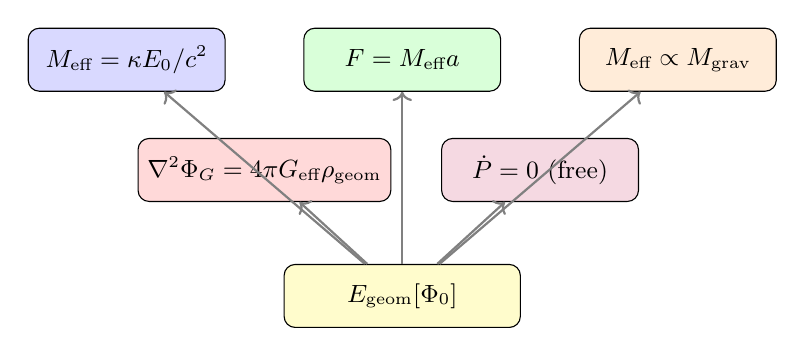
\begin{tikzpicture}[
    box/.style={draw, rounded corners, minimum width=2.5cm, minimum height=0.8cm, align=center, font=\small}
]
    % Results
    \node[box, fill=blue!15] (m1) at (-3.5,2.2) {$\Meff = \kappa E_0/c^2$};
    \node[box, fill=green!15] (m2) at (0,2.2) {$F = \Meff a$};
    \node[box, fill=orange!15] (m3) at (3.5,2.2) {$\Meff \propto \Mgrav$};
    \node[box, fill=red!15] (m4) at (-1.75,0.8) {$\nabla^2\PhiG = 4\pi \Geff\rhogeom$};
    \node[box, fill=purple!15] (m5) at (1.75,0.8) {$\dot{P} = 0$ (free)};
    % Central
    \node[box, fill=yellow!20, minimum width=3cm] (central) at (0,-0.8) {$\Egeom[\Phi_0]$};
    % Arrows
    \foreach \n in {m1, m2, m3, m4, m5} {
        \draw[gray, thick, ->] (central) -- (\n);
    }
\end{tikzpicture}
\caption{Summary schematic: All BP4 results derive from the geometric energy functional $\Egeom[\Phi_0]$. Mass, inertia, force response, gravity, and the proportionality $\Meff \propto \Mgrav$ (basis for equivalence) emerge from a single common origin.}
\label{fig:summary}
\end{figure}

%==============================================================================
% Acknowledgements
%==============================================================================

\section*{Acknowledgements}

This work builds on the foundational analyses of BP3 and BP3.5. The author thanks colleagues and correspondents who provided feedback on earlier drafts. This research was conducted under the auspices of the Vibrational Field Dynamics Institute.

%==============================================================================
% References
%==============================================================================

\begin{thebibliography}{99}

\bibitem{BP3}
L.~Smart, ``Bridge Paper 3: Gravity from Geometric Non-Closure---A $\varphi$-Scaled Scalar-Attractor Framework for Curvature, Entropy, and the Arrow of Time,'' Vibrational Field Dynamics Institute, December 2025.

\bibitem{BP35}
L.~Smart, ``On the Geometric Origin of Matter in Emergent Gravity Frameworks (BP3.5),'' Vibrational Field Dynamics Institute, December 2025.

\bibitem{Manton}
N.~S.~Manton, ``A Remark on the Scattering of BPS Monopoles,'' \textit{Phys. Lett. B} \textbf{110}, 54--56 (1982).

\bibitem{Rajaraman}
R.~Rajaraman, \textit{Solitons and Instantons}, North-Holland, Amsterdam, 1982.

\bibitem{Vilenkin}
A.~Vilenkin and E.~P.~S.~Shellard, \textit{Cosmic Strings and Other Topological Defects}, Cambridge University Press, 1994.

\bibitem{Regge}
T.~Regge, ``General Relativity Without Coordinates,'' \textit{Il Nuovo Cimento} \textbf{19}, 558--571 (1961).

\bibitem{Wald}
R.~M.~Wald, \textit{General Relativity}, University of Chicago Press, 1984.

\bibitem{Goldstein}
H.~Goldstein, C.~Poole, and J.~Safko, \textit{Classical Mechanics}, 3rd ed., Addison-Wesley, 2002.

\bibitem{Will}
C.~M.~Will, ``The Confrontation between General Relativity and Experiment,'' \textit{Living Rev. Relativity} \textbf{17}, 4 (2014).

\bibitem{MICROSCOPE}
P.~Touboul \textit{et al.}, ``MICROSCOPE Mission: Final Results of the Test of the Equivalence Principle,'' \textit{Phys. Rev. Lett.} \textbf{129}, 121102 (2022).

\end{thebibliography}

%==============================================================================
% Appendices
%==============================================================================

\appendix

\section{Details of the Collective Coordinate Derivation}
\label{app:collective}

We provide additional details for the collective coordinate derivation of Section~4.

\subsection{Full Action with Collective Coordinate}

The action for the field $\Phi$ is:
\begin{equation}
    S[\Phi] = \int \dd t \int \dd^3 x \left[ \frac{1}{2c^2}(\partial_t \Phi)^2 - \frac{1}{2}|\nabla \Phi|^2 - \frac{V(\Phi)}{c^2} \right].
\end{equation}

Note: We use conventions where the kinetic term has coefficient $1/(2c^2)$ to give $\Phi$ dimensions of $[\text{energy}]^{1/2}$ and $V$ dimensions of $[\text{energy}/\text{volume}]$.

Substituting $\Phi(\mathbf{x}, t) = \Phi_0(\mathbf{x} - \mathbf{X}(t))$:
\begin{align}
    \partial_t \Phi &= -\dot{X}^i \partial_i \Phi_0, \\
    (\partial_t \Phi)^2 &= \dot{X}^i \dot{X}^j \partial_i \Phi_0 \partial_j \Phi_0.
\end{align}

For an isotropic configuration:
\begin{equation}
    \int \partial_i \Phi_0 \partial_j \Phi_0 \, \dd^3 x = \frac{1}{3}\delta_{ij} \int |\nabla \Phi_0|^2 \, \dd^3 x.
\end{equation}

Thus:
\begin{equation}
    \int \frac{1}{2c^2}(\partial_t \Phi)^2 \, \dd^3 x = \frac{|\dot{\mathbf{X}}|^2}{2c^2} \cdot \frac{1}{3} \int |\nabla \Phi_0|^2 \, \dd^3 x = \frac{1}{2}\Meff |\dot{\mathbf{X}}|^2,
\end{equation}
where:
\begin{equation}
    \Meff = \frac{1}{3c^2} \int |\nabla \Phi_0|^2 \, \dd^3 x.
\end{equation}

\subsection{Higher-Order Corrections}

The $\order{\dot{X}^4/c^4}$ terms in~\eqref{eq:Leff} arise from:
\begin{enumerate}[label=(\roman*)]
    \item Relativistic corrections: Lorentz contraction of the configuration profile;
    \item Internal deformation: Shape changes at high velocity.
\end{enumerate}

These are suppressed by factors of $v^2/c^2$ and can be neglected in the non-relativistic regime $v \ll c$.

\section{Stability Analysis}
\label{app:stability}

\subsection{Spectral Condition for Stability}

The second variation of the energy functional around $\Phi_0$ is:
\begin{equation}
    \delta^2 \Egeom = \int \dd^3 x \, \eta(\mathbf{x}) \mathcal{O} \eta(\mathbf{x}),
\end{equation}
where $\mathcal{O} = -c^2\nabla^2 + V''(\Phi_0(\mathbf{x}))$ is the fluctuation operator.

Stability requires that $\mathcal{O}$ have no negative eigenvalues. For the kink solution with $V(\Phi) = \frac{\lambda}{4}(\Phi^2 - v^2)^2$:
\begin{equation}
    V''(\Phi_0) = \lambda(3\Phi_0^2 - v^2) = \lambda v^2(3\tanh^2(x/\xi) - 1) = 2\lambda v^2\left(1 - \frac{3}{2}\text{sech}^2(x/\xi)\right).
\end{equation}

The operator:
\begin{equation}
    \mathcal{O} = -c^2\frac{\dd^2}{\dd x^2} + 2\lambda v^2 - 3\lambda v^2 \text{sech}^2(x/\xi),
\end{equation}
is a P\"oschl-Teller potential with known spectrum. The ground state has eigenvalue zero (the translational zero mode $\eta_0 \propto \partial_x\Phi_0$), and all other eigenvalues are positive, confirming stability.

\subsection{Zero Modes and Collective Coordinates}

The zero mode corresponds to infinitesimal translation:
\begin{equation}
    \eta_0(x) \propto \frac{\dd\Phi_0}{\dd x} = \frac{v}{\xi}\text{sech}^2(x/\xi).
\end{equation}

Promoting this mode to a collective coordinate $X(t)$ removes the zero mode from the fluctuation spectrum, leaving only massive (stable) modes. This is the standard collective coordinate / moduli space approximation~\cite{Manton}.

\section{Notation Summary}
\label{app:notation}

\begin{table}[H]
\centering
\begin{tabular}{ll}
\toprule
\textbf{Symbol} & \textbf{Meaning} \\
\midrule
$\Phi, \Phi_0$ & Geometric field (order parameter), static configuration \\
$\Egeom$ & Geometric energy functional \\
$E_0$ & Rest energy of stabilised configuration \\
$\varepsilon(\mathbf{x})$ & Energy density of configuration \\
$\Meff$ & Effective inertial mass \\
$\Mgrav$ & Gravitational mass, $= E_0/c^2$ \\
$\kappa$ & Geometric factor, $\Meff = \kappa\Mgrav$ \\
$\mathbf{X}(t)$ & Collective coordinate (centre position) \\
$\dot{\mathbf{X}}$ & Collective coordinate velocity \\
$\Leff$ & Effective Lagrangian \\
$\PhiG$ & Gravitational potential \\
$\rhogeom$ & Geometric mass density, $= \varepsilon/c^2$ \\
$\Geff$ & Effective gravitational constant ($\to G$ in IR) \\
$V(\Phi)$ & Stabilising potential \\
$\xi$ & Characteristic width of configuration \\
$\ell$ & Coherence/discrete scale (from BP3) \\
$v$ & Vacuum expectation value \\
$\lambda$ & Coupling constant in potential \\
$q$ & Abstract configuration parameter \\
\bottomrule
\end{tabular}
\caption{Summary of notation used in this paper.}
\end{table}

\end{document}
